\chapter{Overview of Modern Control Techniques}\label{ch:overview}
This chapter is a general review of the history of adaptive control to include its use cases and previous pitfalls.  A brief overview of algorithm differences between conventional feedback control and \ac{MRAC} architectures is also covered.
%---------------------------------------------------------
\section{Adaptive Control History}\label{history}
Adaptive control saw its early debut in the NASA North American X-15 hypersonic rocket-powered X-plane experimental aircraft.  The X-15's performance envelope exceeded Mach 6.0 and 300,000 feet \cite{jenkins2000x15specs}.  Engineers realized early on that the linear controllers performed well only at one dynamic pressure, but nowhere near the entire flight envelope.  Scheduling the controller gains with respect to dynamic pressure (gain scheduling) was one method used to help ensure robustness;  the method is still widespread in commercial aviation due to its robustness but requires a significant effort to explore the entire flight envelope.  These non-trivial efforts were what encouraged the exploration of the benefits of adaptive control.

The X-15 program started in 1959 and continued to 1968 flying nearly 200 successful flights \cite{nasa_x15_facts}.  It was considered one of NASA's most successful programs.  The benefit of adaptive control to the X-15 was that the adaptive controller was supposed to adjust the gain parameters online automatically.  If the controller was self-tuning, it could potentially offer increased performance while reducing complexity.  Honeywell implemented the MH-96 adaptive controller in the X-15-3 as a fly-by-wire controller designed to adaptively adjust the damping in pitch and roll with respect to the desired model response.  The goal was to achieve consistent aircraft response regardless of dynamic pressure and other variables.  Dydek et. al comments that during test flights of the MH-96 adaptive control, increased performance was observed especially in the dynamic phases of re-entry over that of the linear fixed gain damping system \cite{dydek2010adaptive}.  These early breakthroughs in adaptive control proved the benefits could be viable aerospace solutions.  However, on November 15, 1967, there was a fatal accident caused by the adaptive controller.  NASA documented that the adaptive controller created an out of control flight situation resulting in dynamic pressures exceeding the structural limits and subsequent breakup of the airframe at 65,000 feet \cite{nasa_x15_facts}.

The turbulent start of adaptive control, as implemented on the X-15 program, was due in large part to the early naive understanding of robustness.  Contemporary robust adaptive control strives to encapsulate these deficiencies of robustness in studies and proofs using Lyapunov stability analysis.  In addition to the developments of rigorous stability analysis tools, a number of unique techniques have also been implemented to increase controller robustness.  One such technique utilizes dead band limits on the model adaptation process to avoid system/measurement noise from causing the un-learning of the states and is called \enquote{dead-zone modification} as proposed by B.B. Peterson and K.S. Narendra \cite{peterson1982bounded}.  Lavretsky and Wise also reference the \enquote{$\sigma$ and $e$ modifications} which adds damping to the adaptation process \cite{lavretsky2013robust}.  The \Lone adaptive control algorithm utilizes a technique which seeks to decouple the adaptation rate from robustness by \enquote{low-pass filtering} the contribution of the fast estimator under the premise that estimating the entire frequency spectrum is overly ambitious and should be limited to the bandwidth of the actuator-plant combination.  Many advances have been made in the adaptive control field over the past few decades, and this research sets out to evaluate a small subset of these techniques in the unforgiving aerospace environment.
%---------------------------------------------------------

\section{Classical Feedback vs Adaptive Control}
Control of a system can be categorized into two required elements;  the requirement to stabilize the system in the presence of:
\begin{enumerate}
 \item disturbances that affect the controlled states and outputs (pitch rate perturbation caused by environmental effects)
 \item disturbances that affect the dynamics of the open loop plant (pitch rate effectiveness with respect to dynamic pressure)
\end{enumerate}
Classical feedback control seeks to resolve disturbances that affect the tracking with respect to state perturbation and assume that the plant dynamics are constant.  This form of control is meticulously tuned to achieve the desired overshoot and settling time for example.  The important assumption that is made by classical feedback controllers is that the underlying plant/system dynamics are not changing.  For example, the cruise control that maintains a vehicle's speed assumes that the available horsepower of the car is fixed.  This is a fairly good assumption as the horsepower with respect to rpm available at sea level and 5,000 feet for an internal combustion engine is constant enough that a fixed gain feedback controller would perform well at maintaining the speed of the vehicle in both environments.  In the case of an airplane, the dynamic pressure is proportional to velocity squared and can drastically change the performance of the aircraft.  In this case, the constant system performance assumption can cause a fixed gain classical feedback controller to go unstable at higher dynamic pressures (higher airspeeds).   Conversely, adaptive controllers assume that the system performance is unknown and is likely to vary with time.  Adaptive control seeks to ensure a system's performance with respect to characteristics, such as damping ratio and settling time, which are kept constant regardless of a plant's dynamics that may be unknown and time varying.  For both classical and adaptive control, there exists some form of error which drives the controller.  In the case of classical feedback, the error is calculated between the command and the feedback state of the plant. In adaptive control (in general), the error is calculated between the outputs of the desired reference model and real plant's measured performance.

Figure~\ref{fig:why_adaptive_control} outlines the decision making process a controls engineer makes when deciding the type of controller needed for a given circumstance.

\begin{figure}[h!]
 \centering
  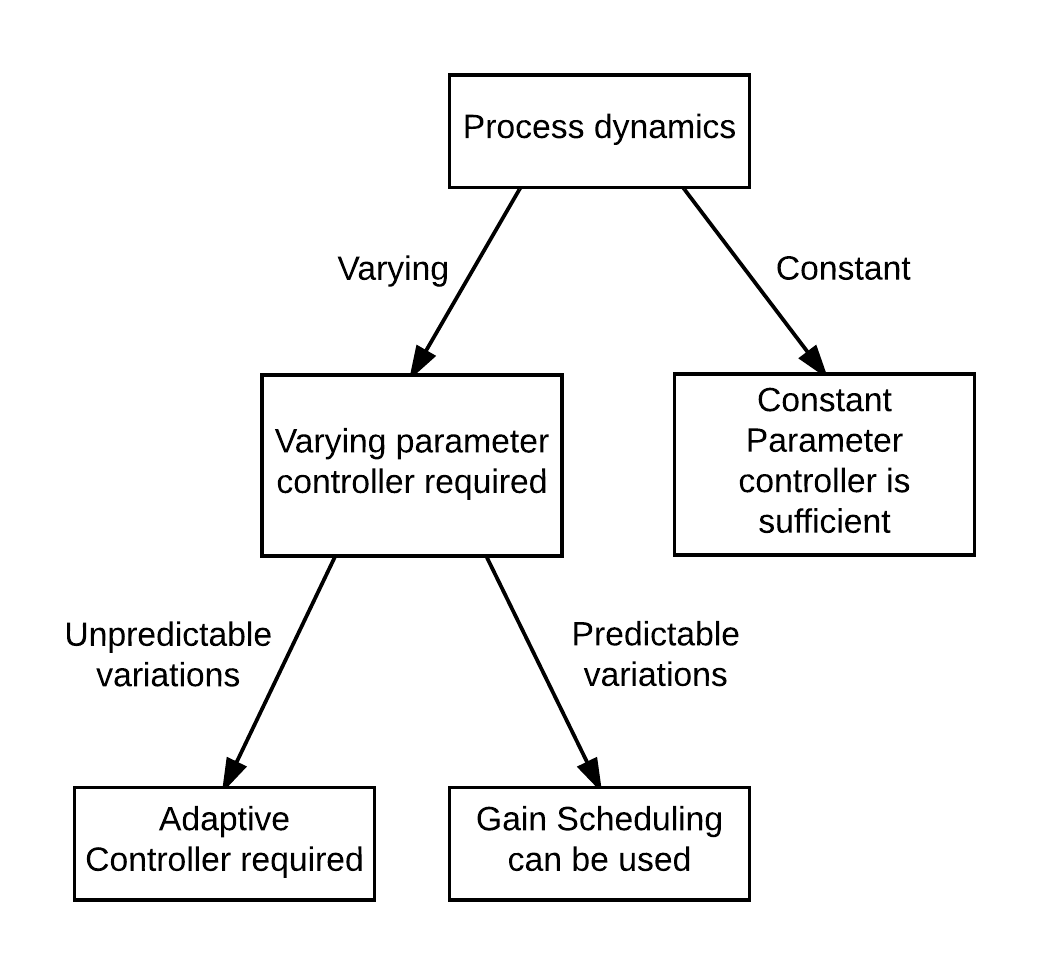
\includegraphics[width=0.5\textwidth]{why_adaptive_control.png}
  \caption{Determine if Adaptive Control Should be Used Adapted from:\cite{aastrom2013adaptive}}
  \label{fig:why_adaptive_control}
\end{figure}


%---------------------------------------------------------
\section{Model Reference Adaptive Control}
\ac{MRAC} establishes the foundation for most of modern, robust adaptive control.  Its structure is intuitive in nature and seeks to define a system's response to a command signal with a reference model.  Unlike traditional feedback where the error signal is generated with respect to state or output error, \ac{MRAC}'s objective is to minimize the error between the performance characteristics of a chosen reference model and the plant.  The error between the model response and the system response generates error for an \enquote{adjustment mechanism} to learn the unknown model parameters.

Figure~\ref{fig:traditional_mrac} illustrates a topology where a traditional feedback controller is established as an inner loop and the \enquote{Reference Model} and \enquote{Adjustment Mechanism} is established as an outer loop.
\begin{figure}[h!]
 \centering
  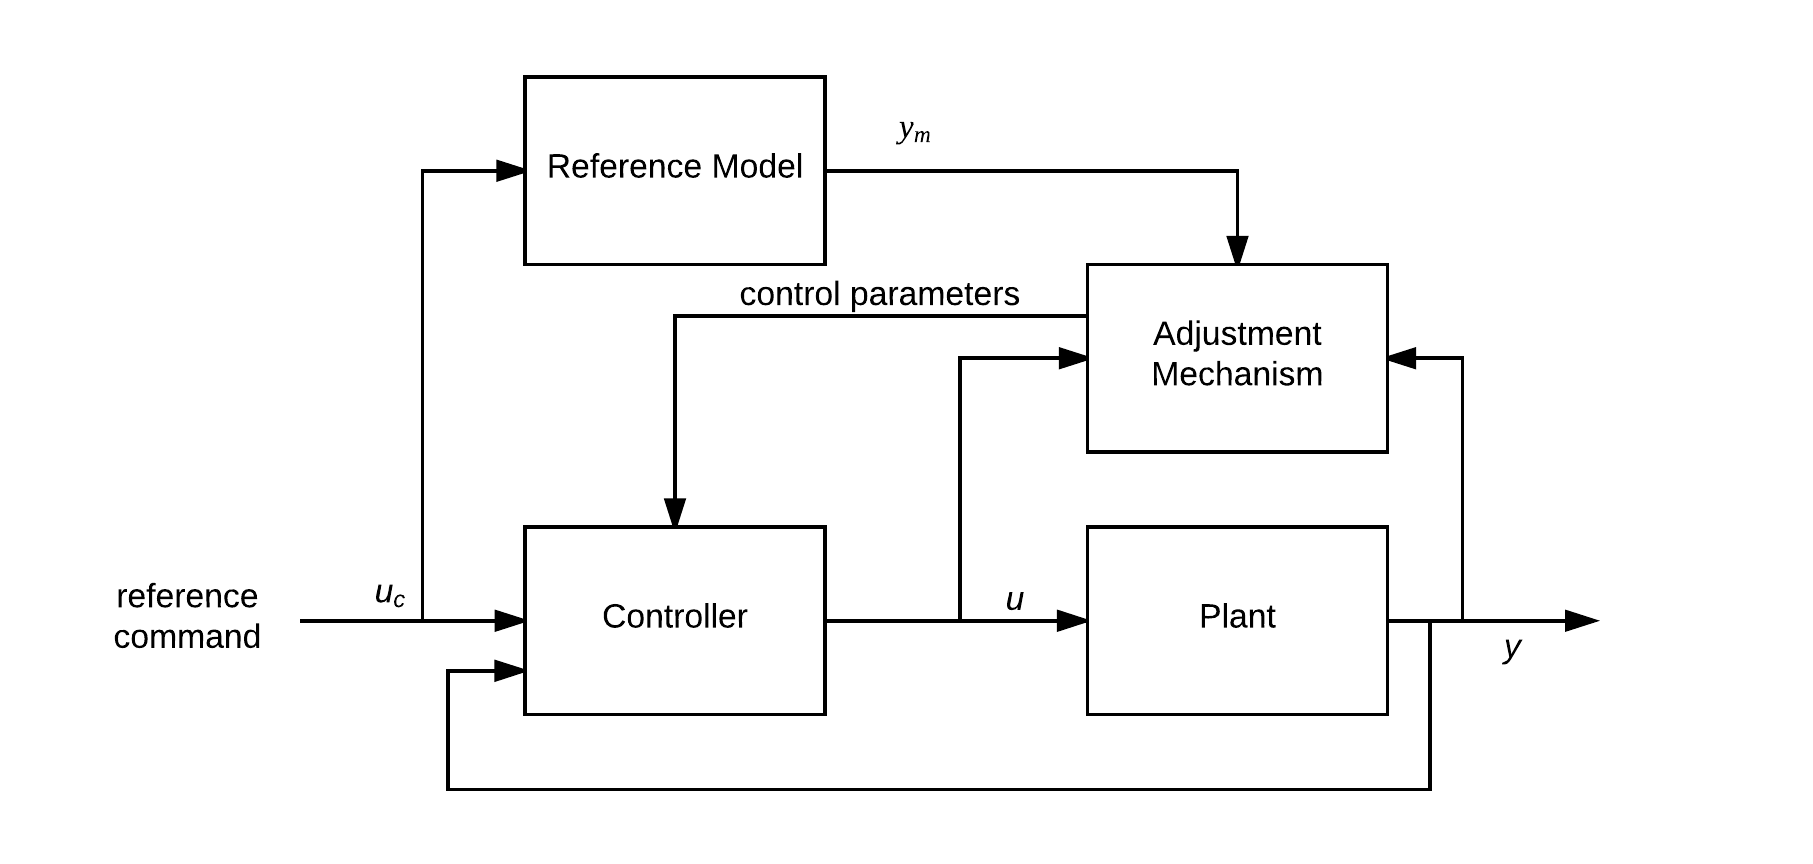
\includegraphics[width=1.0\textwidth]{traditional_MRAC.png}
  \caption{Traditional \ac{MRAC} Architecture Adapted from:\cite{aastrom2013adaptive}}
  \label{fig:traditional_mrac}
\end{figure}
The outer loop attempts to minimize the error between the reference model output and the plant output.  Two primary methods for using this error to learn the system parameters are: gradient descent and Lyapunov stability theory.

\subsection{MIT Rule - Gradient Descent}
One of the first approaches to the design of \ac{MRAC} controllers was implemented at the Instrument Labs at MIT (now known as Draper Labs).  The gradient descent based method was called the \enquote{MIT Rule} for this reason \cite{aastrom2013adaptive}.  This method attempts to learn some unknown parameter by descending the gradient of the error between the reference model and the plant output.

Given the simple first-order system $G(s)$:
\begin{equation}
G(s) = k_{dc}\frac{1}{s+1}
\end{equation}

where $k_{dc}$ is some unknown feedforward gain.  In the case of the MIT rule, $k_{dc}$ is the parameter to be learned and is defined as $\theta$.  The first step in the MIT rule is to establish a cost (or loss) function.  One example of a cost function $J(\theta)$ is:
\begin{equation}
J(\theta) = \frac{1}{2}e^2
\end{equation}
\begin{equation}
e=y-y_m
\end{equation}

where $e$ is error, $y$ is the plant output, and $y_m$ is the model output.

In order for the cost function to be minimized, the negative gradient of the cost function is calculated and used to correct the a priori estimate.  This method takes the following form where $\gamma$ is the adaptation gain:
\begin{equation}
\frac{d\theta}{dt}=-\gamma \frac{\partial{J}}{\partial{\theta}} =-\gamma e\frac{\partial{e}}{\partial{\theta}}
\end{equation}

The stability of this method is very system dependent and heavily relies on trial and error to ensure the adaptation gain $(\gamma)$ is not too high.  This usually requires low adaptation rates for most systems and may not produce adequate results.  It should also be noted that this method relies on adequate persistence of excitation \cite{aastrom2013adaptive}.  In simple terms, the persistence of excitation condition guarantees some functional correspondence between the error and the unknown parameters $\theta$. If the error signal is sufficiently rich, then the partial derivative is explicitly evaluated by the adaptation process running recursively.  Additionally, gradient descents are subject to local extreme convergence for non-convex manifolds.  Therefore, this method does not explicitly guarantee parameter convergence even though correct steady-state gain is achieved for the closed loop system.  

With the differences between classical feedback control and adaptive control being discussed, the next chapter applies analytical tools to develop a specific adaptive control architecture to address the requirements outlined in Chapter~\ref{ch:intro}.




